

\begin{figure}[htp]
\caption{Medien \& Mediennutzung}\label{fig:MedienMediennutzung}
\centering
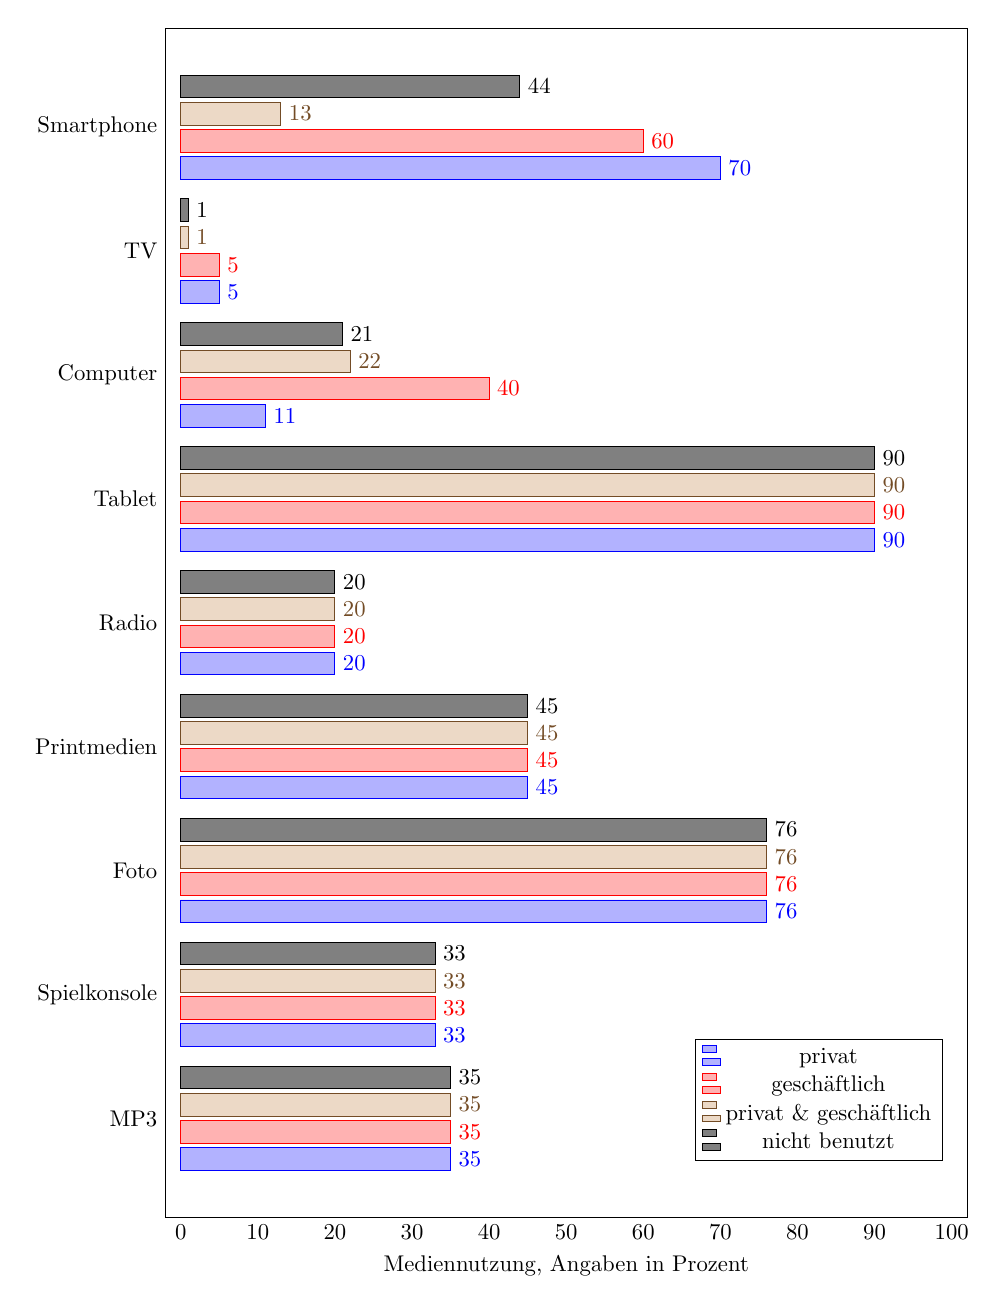
\begin{tikzpicture}[scale=.82, auto,swap]
  \begin{axis}[
    xbar,
    %y axis line style = { opacity = 0 },
    %axis x line       = none,
    tickwidth         = 0pt,
    xmin              = 0,
    xmax              = 100,
    enlarge y limits  = 0.1,
    enlarge x limits  = 0.02,
    %/legend pos=south east,
    legend style={at={(0.97,0.15)}},
    ytick             = data,
    xlabel            = {Mediennutzung, Angaben in Prozent},
    height            = 20cm,
    width             = 14cm,
    symbolic y coords = {MP3, Spielkonsole, Foto, Printmedien, Radio, Tablet, Computer, TV, Smartphone},
    nodes near coords,
    nodes near coords align={horizontal},
  ]
  %privat
  \addplot coordinates { (70,Smartphone)(5,TV)(11,Computer)(90,Tablet)(20,Radio)(45,Printmedien)(76,Foto)(33,Spielkonsole)(35,MP3)};
  %geschäftlich
  \addplot coordinates { (60,Smartphone)(5,TV)(40,Computer)(90,Tablet)(20,Radio)(45,Printmedien)(76,Foto)(33,Spielkonsole)(35,MP3)};
  %privat und geschäftlich
  \addplot coordinates { (13,Smartphone)(1,TV)(22,Computer)(90,Tablet)(20,Radio)(45,Printmedien)(76,Foto)(33,Spielkonsole)(35,MP3)};
  %nicht benutzt
  \addplot coordinates { (44,Smartphone)(1,TV)(21,Computer)(90,Tablet)(20,Radio)(45,Printmedien)(76,Foto)(33,Spielkonsole)(35,MP3)};
  
  
  \legend{privat, geschäftlich, privat \& geschäftlich, nicht benutzt}
  \end{axis}
\end{tikzpicture}
\end{figure}